\section{Introduction}\label{sec:intro}

Automated monitoring of rice pests increasingly relies on object detectors applied to high-resolution light-trap and field images, where the species that matter most for early warning are often the rarest in the catch and the smallest in the frame~\citep{mo2025ricepest,li2026agrisurvey}. Because a detector trained at a fixed input size loses small objects once a multi-megapixel image is downscaled to fit, practitioners tile the image, run the detector on each tile, and merge the per-tile boxes. This sliced-inference recipe, popularised as slicing-aided hyper inference (SAHI) and the tiling that preceded it~\citep{akyon2022sahi,unel2019tiling}, is now standard in agricultural pest pipelines~\citep{fotouhi2024sticky,ye2024teasahi,wei2026yolousw}. It is routinely justified by an intuitive chain: a rare, tail-class species tends to be small; a small object straddling a tile boundary loses its pixels to the cut; and the overlap between adjacent tiles exists precisely to keep such objects whole.

Each link of that chain is asserted rather than measured, and the first two do not hold for long-tailed rice pests. Rarity and smallness are distinct axes: in the primary dataset the head classes carry a \emph{larger} fraction of small objects than the tail does, so ``tail implies small'' is false. Whether a boundary actually removes an object's pixels under standard overlap has, to our knowledge, never been counted per object; the overlap is defended by the possibility of a cut rather than by its measured frequency. If truncation is in fact rare, the usual prescriptions for where to spend effort, such as wider overlap or boundary-aware merging, address a loss that may not exist, and the real question becomes where tail-class small objects are actually lost once size is held apart from frequency.

Existing tools for localising detection errors stop short of that question. Error-decomposition frameworks attribute final-output mistakes to classification, localisation or duplication, but they analyse the boxes a detector emits and never ask whether a matching candidate was formed in the first place~\citep{hoiem2012diagnosing,bolya2020tide}. Analyses specific to sliced inference examine the merge: cross-view agreement rescoring, for example, improves tiled detection by re-ranking boxes that already exist across tiles~\citep{na2026crossview}, which presupposes a surviving candidate. Long-tailed detection methods re-weight or recalibrate decoded scores~\citep{pan2021norcal,alexandridis2025fracal} or adjust the output cap that discards low-ranked boxes~\citep{dave2021devil}, again operating only on what reached the scored list. None of these reports, per ground-truth object and with class frequency separated from object size, the pipeline stage at which a tail-class small object is lost, which is the single fact that decides whether any of these remedies can reach it.

We close that gap with a pre-registered, group-held-out, size-controlled audit of sliced inference on frozen detectors. The detector and its slicing geometry are fixed before any audit result is inspected; every per-tile candidate is dumped at a permissive score floor; and each ground-truth object is traced through a five-stage ledger, namely tile coverage, candidate formation, cross-tile merge, score threshold and output cap, so that each miss is charged to the stage that first removed it and sorted into a recovery-ceiling category that names the class of fix it admits (Fig.~\ref{fig:roadmap}; the instrument is detailed in Fig.~\ref{fig:arch}). The organising insight is that locating a loss is more actionable than any single remedy: once a miss is known to have no candidate in any view, every post-hoc fix is ruled out for it, and effort belongs in the detector or its training instead. On a group-disjoint audit set we find that literal boundary truncation is negligible, that a majority of tail-small misses have no candidate in any view, that this difference from same-size head classes survives size matching, and that a class-conditional read-out adds nothing over calibration; the slice boundary is, in this setting, a secondary contributor, and the tail-small ceiling is set at candidate formation.

\begin{figure}[!htbp]
    \centering
    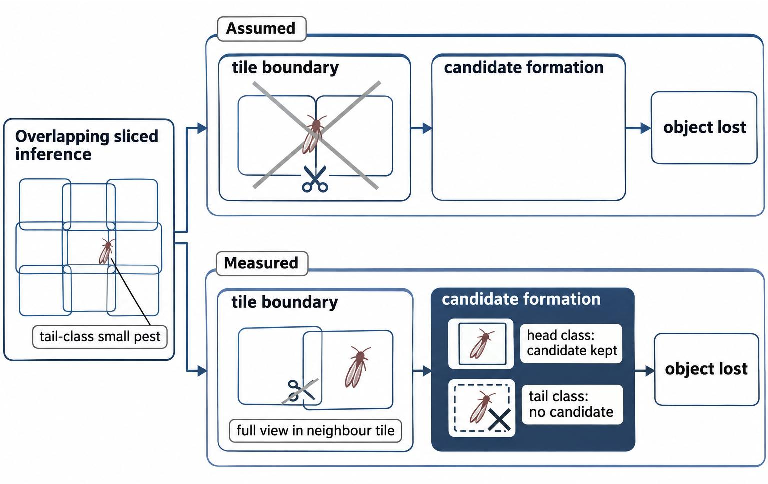
\includegraphics[width=0.98\textwidth,height=0.8\textheight,keepaspectratio]{../figures/fig_roadmap.pdf}
    \caption{The assumed slice-boundary loss (a tail-class small pest cut by a tile seam and lost) versus the measured loss for long-tailed small rice pests: a full view exists in a neighbouring tile, and the loss occurs earlier, at candidate formation.}
    \label{fig:roadmap}
\end{figure}

Concretely, this paper contributes (i) a measured negative control showing that literal truncation is negligible under standard overlap, with none of the 38 tail-small objects lacking a full view (Section~\ref{sec:res-trunc}, Fig.~\ref{fig:truncation}), against the unmeasured overlap rationale of the sliced-inference literature~\citep{akyon2022sahi,unel2019tiling}; (ii) a pre-registered recovery-ceiling partition that localises the pooled tail-small loss to candidate formation on the primary detector and names which class of fix is admissible there (Section~\ref{sec:res-partition}, Table~\ref{tab:partition}, Fig.~\ref{fig:partition}), relative to output-only error decomposition~\citep{hoiem2012diagnosing,bolya2020tide} and merge-stage-only slicing analyses~\citep{na2026crossview}; (iii) a size-versus-frequency dissociation, confirmed by a size-matched contrast (Section~\ref{sec:res-contrast}, Fig.~\ref{fig:contrast}), showing the tail-small loss is not accounted for by object size, against long-tail framing that treats rarity and smallness together~\citep{pan2021norcal}; and (iv) a pre-registered class-conditional read-out reported as a negative increment (Section~\ref{sec:res-methods}, Table~\ref{tab:ccpr}), with the dominant loss stage shown to be contingent on the detector and the image source (Sections~\ref{sec:res-detector}--\ref{sec:res-yst}). The audit is deliberately a measurement rather than a new detector, and its product is a map of which class of fix each loss admits rather than a benchmark score.
